\chapter{System Design}

\section{System Architecture}
The system architecture of \textbf{StepCharge AI} follows an end-to-end cyber-physical design structured into five decoupled operational tiers: Edge Hardware, Embedded Firmware, Cloud Backend, Machine Learning Microservice, and Presentation Client. Figure~\ref{fig:system_architecture} illustrates the architectural topology and multi-protocol dataflow connecting physical footstep impacts to real-time client visualization.

\begin{figure}[H]
\centering
\begin{tikzpicture}[
    scale=0.85, every node/.style={scale=0.85},
    node distance=1.5cm,
    block/.style={rectangle, rounded corners=6pt, draw=black!80, thick, fill=blue!8, align=center, minimum width=3.2cm, minimum height=1.0cm, font=\small},
    subblock/.style={rectangle, rounded corners=4pt, draw=black!70, fill=white, align=center, minimum width=2.8cm, minimum height=0.75cm, font=\footnotesize},
    container/.style={rectangle, rounded corners=8pt, draw=black!60, dashed, thick, fill=gray!5, inner sep=12pt},
    arrow/.style={-{Latex[length=2.5mm]}, thick, draw=blue!80!black},
    darrow/.style={{Latex[length=2mm]}-{Latex[length=2mm]}, thick, draw=purple!80!black}
]
    % Edge Hardware Tier
    \node (piezo) [block, fill=teal!15] {\textbf{Piezo Tile Array}\\(8$\times$ PZT-5 Discs)};
    \node (rect) [block, fill=teal!15, right=1.0cm of piezo] {\textbf{Schottky Rectifier}\\\& 5.1V Zener Clamp};
    \node (cap) [block, fill=teal!15, right=1.0cm of rect] {\textbf{Supercapacitor}\\(0.1F / 5.5V Buffer)};

    % Embedded Tier
    \node (esp) [block, fill=amber!15, below=1.8cm of rect] {\textbf{ESP32 Microcontroller}\\Core 0: Wi-Fi / HTTPS\\Core 1: 50Hz ADC \& Filter};
    \node (loads) [block, fill=teal!15, right=1.0cm of esp] {\textbf{Demonstration Loads}\\LED / DC Fan (MOSFETs)};

    % Cloud Backend Tier
    \node (backend) [block, fill=blue!15, below=1.8cm of esp] {\textbf{Node.js + Express API}\\(:5000) REST / Auth};
    \node (mongo) [block, fill=green!15, left=1.2cm of backend] {\textbf{MongoDB Atlas}\\Time-Series Database};
    \node (socket) [block, fill=cyan!15, right=1.2cm of backend] {\textbf{Socket.IO Gateway}\\Real-Time Broadcaster};

    % ML and Frontend Tier
    \node (ml) [block, fill=purple!15, below=1.8cm of mongo] {\textbf{FastAPI ML Service}\\(:8000) Random Forest};
    \node (frontend) [block, fill=orange!15, below=1.8cm of socket] {\textbf{React 19 Dashboard}\\(:5173) Live Telemetry};

    % Connecting Arrows
    \draw [arrow] (piezo) -- node [above, font=\scriptsize] {AC Kinetic} (rect);
    \draw [arrow] (rect) -- node [above, font=\scriptsize] {DC Charge} (cap);
    \draw [arrow] (rect) |- node [left, pos=0.7, font=\scriptsize] {Pulse (GPIO 34)} (esp);
    \draw [arrow] (cap) |- node [right, pos=0.7, font=\scriptsize] {Storage (GPIO 35)} (esp);
    \draw [darrow] (esp) -- node [above, font=\scriptsize] {Gate / Readback} (loads);

    \draw [arrow] (esp) -- node [right, font=\scriptsize] {HTTPS Telemetry / Keys} (backend);
    \draw [darrow] (backend) -- node [above, font=\scriptsize] {Mongoose ODM} (mongo);
    \draw [arrow] (backend) -- node [above, font=\scriptsize] {Telemetry Events} (socket);

    \draw [darrow] (backend) |- node [above, pos=0.7, font=\scriptsize] {POST /predict} (ml);
    \draw [arrow] (socket) -- node [right, font=\scriptsize] {WSS / Event Stream} (frontend);
    \draw [darrow] (frontend) -| node [below, pos=0.25, font=\scriptsize] {REST Commands / Google Auth} (backend);

\end{tikzpicture}
\caption{Overall StepCharge AI multi-tier cyber-physical system architecture.}
\label{fig:system_architecture}
\end{figure}

The architecture ensures that analog sensing and power conditioning remain completely decoupled from high-level cloud services. Even during transient network outages, local energy accumulation and step detection continue uninterrupted on the edge hardware.

\section{Overall Hardware Architecture}
The hardware subsystem integrates kinetic energy harvesting, analog conditioning, digital processing, and power switching. Figure~\ref{fig:hardware_block_diagram} provides a structural block diagram of the physical components.

\begin{figure}[H]
\centering
\begin{tikzpicture}[
    scale=0.88, every node/.style={scale=0.88},
    block/.style={rectangle, rounded corners=5pt, draw=black!80, thick, fill=blue!8, align=center, minimum width=2.8cm, minimum height=0.9cm, font=\small},
    arrow/.style={-{Latex[length=2.5mm]}, thick, draw=black!80}
]
    \node (p1) [block, fill=teal!15] {PZT Array\\(8 Ceramic Discs)};
    \node (rec) [block, fill=cyan!15, right=1.0cm of p1] {Schottky Bridge\\(1N5819 $\times$4)};
    \node (tvs) [block, fill=red!15, right=1.0cm of rec] {Zener Clamp\\(5.1V TVS)};
    \node (cap) [block, fill=teal!20, right=1.0cm of tvs] {Supercapacitor\\(0.1F / 5.5V)};

    \node (div1) [block, fill=yellow!15, below=1.2cm of rec] {Pulse Divider\\(2:1 Ratio)};
    \node (div2) [block, fill=yellow!15, below=1.2cm of cap] {Storage Divider\\(2:1 Ratio)};

    \node (esp) [block, fill=amber!20, minimum width=5.5cm, below=1.2cm of div1, xshift=2.0cm] {\textbf{Espressif ESP32-WROOM-32D}\\ADC1\_CH6 (GPIO 34) $\cdot$ ADC1\_CH7 (GPIO 35)\\GPIO 25 (LED Gate) $\cdot$ GPIO 26 (Fan Gate)};

    \node (mos) [block, fill=orange!15, below=1.2cm of esp] {MOSFET Drivers\\(IRLZ44N $\times$2)};
    \node (load) [block, fill=green!15, right=1.0cm of mos] {Demonstration Loads\\LED \& 5V DC Fan};

    \draw [arrow] (p1) -- (rec);
    \draw [arrow] (rec) -- (tvs);
    \draw [arrow] (tvs) -- (cap);
    \draw [arrow] (rec) -- (div1);
    \draw [arrow] (cap) -- (div2);
    \draw [arrow] (div1) -- (esp.north -| div1);
    \draw [arrow] (div2) -- (esp.north -| div2);
    \draw [arrow] (esp) -- (mos);
    \draw [arrow] (mos) -- (load);

\end{tikzpicture}
\caption{Detailed hardware block diagram of the StepCharge AI edge harvesting node.}
\label{fig:hardware_block_diagram}
\end{figure}

\section{Piezoelectric Energy Harvesting Subsystem}
The harvesting array consists of 8 commercial 35\,mm circular Lead Zirconate Titanate (PZT-5) diaphragm elements mounted onto flexible brass backing plates. The transducers are wired in a series-parallel matrix ($2 \times 4$) embedded within an elastomeric polyurethane frame beneath a rigid $300\,\text{mm} \times 300\,\text{mm}$ acrylic top plate. When a footstep impact lands on the plate, mechanical force is distributed across the ceramic elements, inducing dynamic flexural bending and generating simultaneous charge outputs.

\section{Rectifier and Power Conditioning Circuit}
Because piezoelectric transducers generate bipolar alternating current (AC), rectification is mandatory. Figure~\ref{fig:circuit_diagram} depicts the electrical circuit schematic of the conditioning and measurement stages.

\begin{figure}[H]
\centering
\begin{tikzpicture}[
    scale=0.88, every node/.style={scale=0.88},
    circuit/.style={draw=black!80, thick},
    comp/.style={rectangle, draw=black!80, thick, fill=white, align=center, inner sep=4pt, font=\scriptsize}
]
    % Input from Piezo
    \draw [circuit] (0,2) node[left] {Piezo (+)} -- (1.5,2);
    \draw [circuit] (0,0) node[left] {Piezo (-)} -- (1.5,0);

    % Bridge Rectifier
    \draw [circuit] (1.5,1) rectangle (3.5,3) node[pos=0.5, font=\scriptsize, align=center] {Schottky\\Bridge\\(4$\times$ 1N5819)};
    \draw [circuit] (1.5,2) -- (1.5,1);
    \draw [circuit] (1.5,0) |- (2.5,1);

    % Rectified Output
    \draw [circuit] (3.5,2) -- (5.0,2) node[circle, fill=black, inner sep=1.5pt] (p1) {};
    \draw [circuit] (2.5,1) |- (5.0,0) node[circle, fill=black, inner sep=1.5pt] (g1) {};

    % Zener / TVS Clamp
    \draw [circuit] (5.0,2) -- (6.0,2) node[circle, fill=black, inner sep=1.5pt] (p2) {};
    \draw [circuit] (5.0,0) -- (6.0,0) node[circle, fill=black, inner sep=1.5pt] (g2) {};
    \draw [circuit] (p2) -- (6.0,1.4) node[comp] {5.1V\\Zener} -- (g2);

    % Supercapacitor
    \draw [circuit] (6.0,2) -- (8.0,2) node[circle, fill=black, inner sep=1.5pt] (p3) {};
    \draw [circuit] (6.0,0) -- (8.0,0) node[circle, fill=black, inner sep=1.5pt] (g3) {};
    \draw [circuit] (p3) -- (8.0,1.4) node[comp] {0.1F\\5.5V} -- (g3);

    % Voltage Divider to ADC (Storage)
    \draw [circuit] (8.0,2) -- (10.0,2);
    \draw [circuit] (10.0,2) -- (10.0,1.4) node[comp] {$R_1$\\$100\text{k}\Omega$} -- (10.0,0.8) node[circle, fill=black, inner sep=1.5pt] (adc2) {} -- (10.0,0.4) node[comp] {$R_2$\\$100\text{k}\Omega$} -- (10.0,0);
    \draw [circuit] (8.0,0) -- (10.0,0) node[below, font=\scriptsize] {GND};
    \draw [circuit, -{Latex}] (adc2) -- (11.5,0.8) node[right, font=\scriptsize] {ESP32 GPIO 35 (Storage)};

    % Pulse Divider (Tap from Rectified rail)
    \draw [circuit] (5.0,2) |- (5.0,3.5) -- (6.5,3.5);
    \draw [circuit] (6.5,3.5) -- (6.5,2.9) node[comp] {$R_3$\\$100\text{k}\Omega$} -- (6.5,2.3) node[circle, fill=black, inner sep=1.5pt] (adc1) {} -- (6.5,1.7) node[comp] {$R_4$\\$100\text{k}\Omega$} -- (6.5,1.2) node[below, font=\scriptsize] {GND};
    \draw [circuit, -{Latex}] (adc1) -- (8.0,2.3) node[right, font=\scriptsize] {ESP32 GPIO 34 (Pulse)};

\end{tikzpicture}
\caption{Electrical schematic of rectification, clamping, supercapacitor, and divider sensing.}
\label{fig:circuit_diagram}
\end{figure}

The Schottky diodes (1N5819) exhibit an ultra-low forward-voltage drop ($V_F \approx 0.35\,\text{V}$), conserving scarce micro-energy during low-velocity footfalls. A 5.1\,V Zener clamping diode shunts excessive voltage transients to ground, preventing damage to the supercapacitor buffer and the microcontroller ADC.

\section{Supercapacitor Energy Storage}
Energy accumulation utilizes a 0.1\,F, 5.5\,V Electric Double-Layer Capacitor (EDLC). The total electrical energy stored electrostatically in the capacitor dielectric is given by:
\begin{equation}
E = \frac{1}{2} C V^2
\label{eq:cap_energy}
\end{equation}
where $C = 0.10\,\text{F}$ and $V$ is the terminal voltage. The differential energy accumulated between consecutive footstep cycles is:
\begin{equation}
\Delta E = \frac{1}{2} C \left(V_{\text{final}}^2 - V_{\text{initial}}^2\right)
\label{eq:delta_energy}
\end{equation}

\section{Voltage Measurement Subsystem}
To interface external potentials with the ESP32 ($0.0\text{--}3.3\,\text{V}$ absolute maximum), symmetric $100\,\text{k}\Omega / 100\,\text{k}\Omega$ metal-film resistive dividers are implemented, establishing a scaling ratio of:
\begin{equation}
M = \frac{R_1 + R_2}{R_2} = \frac{100\,\text{k}\Omega + 100\,\text{k}\Omega}{100\,\text{k}\Omega} = 2.0
\label{eq:divider_ratio}
\end{equation}
The true physical voltage $V_{\text{phys}}$ is calculated from the raw 12-bit ADC integer $D \in [0, 4095]$ as:
\begin{equation}
V_{\text{phys}} = \left(\frac{D}{4095.0}\right) \times 3.30\,\text{V} \times 2.0
\label{eq:adc_conversion}
\end{equation}

\section{ESP32 Embedded Monitoring and Signal Acquisition}
The firmware executes a dual-threshold Schmitt trigger to detect valid footsteps. Figure~\ref{fig:schmitt_wave} illustrates the hysteresis detection mechanics.

\begin{figure}[H]
\centering
\begin{tikzpicture}[scale=0.9, every node/.style={scale=0.9}]
    \draw [->, thick] (0,0) -- (9.0,0) node [right] {Time (ms)};
    \draw [->, thick] (0,0) -- (0,4.2) node [above] {Voltage (V)};

    % Threshold lines
    \draw [dashed, red!80, thick] (0,2.4) -- (8.5,2.4) node [right, font=\scriptsize] {$V_{\text{high}} = 0.80\,\text{V}$ (Rising Trigger)};
    \draw [dashed, blue!80, thick] (0,1.65) -- (8.5,1.65) node [right, font=\scriptsize] {$V_{\text{low}} = 0.55\,\text{V}$ (Falling Release)};

    % Simulated pulse waveform
    \draw [thick, green!60!black, smooth] plot coordinates {
        (0.5,0.2) (1.2,0.3) (2.0,0.5) (2.4,1.0) (2.8,2.4) (3.2,3.6) (3.8,3.2) (4.4,2.2) (5.0,1.65) (5.6,0.8) (6.2,0.3) (8.0,0.2)
    };

    % Detection Points
    \node at (2.8,2.4) [circle, fill=red, inner sep=2pt] {};
    \node at (2.8,2.8) [font=\scriptsize, red!80!black] {Pulse Start ($t_{\text{start}}$)};

    \node at (5.0,1.65) [circle, fill=blue, inner sep=2pt] {};
    \node at (5.0,1.2) [font=\scriptsize, blue!80!black] {Pulse End ($t_{\text{end}}$)};

    \node at (3.2,3.6) [circle, fill=orange, inner sep=2pt] {};
    \node at (3.2,4.0) [font=\scriptsize, orange!80!black] {Peak ($V_{\text{peak}} = 3.6\,\text{V}$)};

    % Duration Bracket
    \draw [{Latex}-{Latex}, thick] (2.8,0.5) -- (5.0,0.5) node [midway, above, font=\scriptsize] {$T_{\text{pulse}}$};

    % Refractory Window
    \draw [fill=gray!20, opacity=0.5] (5.0,0) rectangle (7.5,4.0);
    \node at (6.25,2.0) [font=\scriptsize, rotate=90, align=center] {Refractory Lockout\\(250 ms)};

\end{tikzpicture}
\caption{Schmitt-trigger hysteresis detection waveform and refractory lockout window.}
\label{fig:schmitt_wave}
\end{figure}

\section{IoT Communication Architecture}
The edge node communicates with the cloud backend via standard TLS-encrypted HTTPS REST protocols. Edge telemetry frames are published every 1000\,ms via \texttt{POST /api/devices/:id/telemetry}. Discrete footsteps are appended via \texttt{POST /api/devices/:id/footsteps}.

\section{Backend Architecture}
The backend service is structured into modular layers:
\begin{itemize}
    \item \textbf{Routing Layer:} Express routers handling \texttt{/api/auth}, \texttt{/api/devices}, \texttt{/api/telemetry}, \texttt{/api/alerts}, and \texttt{/api/ml}.
    \item \textbf{Middleware Layer:} Cryptographic device key validation (\texttt{requireDeviceAuth}), JWT session verification (\texttt{requireAuth}), RBAC enforcement (\texttt{requireAdmin}), rate limiters, and Helmet headers.
    \item \textbf{Service Layer:} Telemetry persistence, health monitoring, and Socket.IO emission.
\end{itemize}

\section{Database Design}
MongoDB Atlas provides document persistence. Relational integrity is enforced programmatically via Mongoose ODM schemas. The primary entity relationships are shown in Section~\ref{sec:er_diagram}.

\section{Machine Learning Architecture}
The machine learning architecture runs as an independent Python FastAPI microservice. The model takes a 5-element feature vector and classifies it via a Random Forest model. Figure~\ref{fig:ml_workflow} illustrates the end-to-end training and inference pipeline.

\begin{figure}[H]
\centering
\begin{tikzpicture}[
    scale=0.88, every node/.style={scale=0.88},
    stage/.style={rectangle, rounded corners=5pt, draw=black!80, thick, fill=blue!10, align=center, minimum width=2.6cm, minimum height=0.85cm, font=\scriptsize},
    arrow/.style={-{Latex[length=2.5mm]}, thick, draw=blue!80!black}
]
    \node (raw) [stage, fill=teal!15] {Raw ADC Pulse\\$\sigma(t)$ at 50\,Hz};
    \node (filt) [stage, fill=teal!15, right=0.8cm of raw] {Schmitt Detection\\$\&$ Duration Filter};
    \node (feat) [stage, fill=yellow!15, right=0.8cm of filt] {Feature Vector\\$[V_{\text{pk}}, V_{\text{avg}}, T_p, \Delta T, V_s]$};
    \node (rf) [stage, fill=purple!15, right=0.8cm of feat] {Random Forest\\(100 Trees)};
    \node (out) [stage, fill=green!15, right=0.8cm of rf] {Class Prediction\\\& Confidence};

    \node (db) [stage, fill=gray!15, below=1.0cm of feat] {Dataset Repository\\(Stratified GroupKFold)};

    \draw [arrow] (raw) -- (filt);
    \draw [arrow] (filt) -- (feat);
    \draw [arrow] (feat) -- (rf);
    \draw [arrow] (rf) -- (out);
    \draw [arrow] (feat) -- (db);
    \draw [arrow] (db) -| node [pos=0.3, right, font=\tiny] {Trained Model} (rf);

\end{tikzpicture}
\caption{Machine Learning feature extraction, training, and inference workflow.}
\label{fig:ml_workflow}
\end{figure}

\section{Frontend Dashboard Architecture}
The frontend is constructed using React 19 and TypeScript, structured around a global \texttt{StoreProvider}. A custom hook (\texttt{useStore}) connects to the Socket.IO client, dynamically receiving telemetry frames and updating charts without full re-renders.

\section{Data Flow Diagrams}

\subsection{Data Flow Diagram Level 0 (Context Level)}
Figure~\ref{fig:dfd_level0} illustrates the Level 0 Context DFD representing the highest-level interaction between external entities and the StepCharge AI platform.

\begin{figure}[H]
\centering
\begin{tikzpicture}[
    scale=0.88, every node/.style={scale=0.88},
    entity/.style={rectangle, draw=black!80, thick, fill=orange!15, align=center, minimum width=2.5cm, minimum height=1.0cm, font=\small\bfseries},
    process/.style={circle, draw=black!80, thick, fill=blue!15, align=center, minimum size=3.2cm, font=\small\bfseries},
    arrow/.style={-{Latex[length=2.5mm]}, thick, draw=black!80}
]
    \node (esp) [entity] {ESP32 Edge\\Harvester};
    \node (sys) [process, right=2.5cm of esp] {StepCharge AI\\Central System\\(Level 0)};
    \node (user) [entity, right=2.5cm of sys] {Authenticated\\User / Admin};

    \draw [arrow] (esp.north east) -- node [above, font=\scriptsize] {Telemetry \& Steps} (sys.north west);
    \draw [arrow] (sys.south west) -- node [below, font=\scriptsize] {Load Poll / Config} (esp.south east);

    \draw [arrow] (user.north west) -- node [above, font=\scriptsize] {Auth / Control} (sys.north east);
    \draw [arrow] (sys.south east) -- node [below, font=\scriptsize] {Visual Dashboards} (user.south west);

\end{tikzpicture}
\caption{Data Flow Diagram (DFD) Level 0 --- Context Level Diagram.}
\label{fig:dfd_level0}
\end{figure}

\subsection{Data Flow Diagram Level 1}
Figure~\ref{fig:dfd_level1} decomposes the system into discrete functional processes, illustrating data stores and internal data paths.

\begin{figure}[H]
\centering
\begin{tikzpicture}[
    scale=0.82, every node/.style={scale=0.82},
    entity/.style={rectangle, draw=black!80, thick, fill=orange!15, align=center, minimum width=2.2cm, minimum height=0.9cm, font=\scriptsize\bfseries},
    proc/.style={circle, draw=black!80, thick, fill=blue!12, align=center, minimum size=2.2cm, font=\scriptsize\bfseries},
    store/.style={rectangle, draw=black!80, thick, fill=yellow!15, minimum width=2.6cm, minimum height=0.7cm, font=\scriptsize\bfseries},
    arrow/.style={-{Latex[length=2.2mm]}, thick, draw=black!80}
]
    % Entities
    \node (esp) [entity] at (0, 6) {ESP32 Edge\\Node};
    \node (user) [entity] at (12, 6) {Web Client\\User};

    % Processes
    \node (p1) [proc] at (3.5, 6) {1.0\\Ingest \& Verify\\Telemetry};
    \node (p2) [proc] at (8.5, 6) {2.0\\Authenticate\\\& Authorize};
    \node (p3) [proc] at (3.5, 2.5) {3.0\\Execute ML\\Inference};
    \node (p4) [proc] at (8.5, 2.5) {4.0\\Manage Closed\\Loop Loads};
    \node (p5) [proc] at (6.0, -0.5) {5.0\\Real-Time Event\\Broadcast};

    % Data Stores
    \node (d1) [store] at (6.0, 4.2) {D1: Telemetry Collection};
    \node (d2) [store] at (6.0, 1.2) {D2: Footsteps Collection};
    \node (d3) [store] at (12, 2.5) {D3: Users \& Devices};

    % Data Flows
    \draw [arrow] (esp) -- node [above, font=\tiny] {Raw Frames} (p1);
    \draw [arrow] (p1) -- node [above, font=\tiny] {Write} (d1);
    \draw [arrow] (p1) -- node [left, font=\tiny] {Step Vector} (p3);
    \draw [arrow] (p3) -- node [above, font=\tiny] {Persist Class} (d2);
    \draw [arrow] (user) -- node [above, font=\tiny] {Login / JWT} (p2);
    \draw [arrow] (p2) -- node [right, font=\tiny] {Verify} (d3);
    \draw [arrow] (user) -- node [right, font=\tiny] {Load Intent} (p4);
    \draw [arrow] (p4) -- node [above, font=\tiny] {Poll State} (esp);
    \draw [arrow] (d1) -- (p5);
    \draw [arrow] (d2) -- (p5);
    \draw [arrow] (p5) -| node [below, pos=0.25, font=\tiny] {Socket.IO Push} (user);

\end{tikzpicture}
\caption{Data Flow Diagram (DFD) Level 1 --- Functional Process Decomposition.}
\label{fig:dfd_level1}
\end{figure}

\section{Entity Relationship Diagram}
\label{sec:er_diagram}
Figure~\ref{fig:er_diagram} presents the Entity-Relationship (ER) model defining the primary collections, attributes, and cardinality in MongoDB Atlas.

\begin{figure}[H]
\centering
\begin{tikzpicture}[
    scale=0.82, every node/.style={scale=0.82},
    entity/.style={rectangle, draw=black!80, thick, fill=blue!15, align=center, minimum width=2.4cm, minimum height=0.9cm, font=\scriptsize\bfseries},
    attr/.style={ellipse, draw=black!70, fill=gray!10, align=center, font=\tiny, inner sep=2pt},
    rel/.style={diamond, draw=black!80, thick, fill=orange!15, align=center, font=\tiny\bfseries, inner sep=2pt},
    line/.style={thick, draw=black!70}
]
    % Entities
    \node (user) [entity] at (0, 4) {User};
    \node (dev) [entity] at (5, 4) {Device};
    \node (telem) [entity] at (10, 4) {Telemetry};
    \node (step) [entity] at (5, 0) {Footstep};

    % Relationships
    \node (r1) [rel] at (2.5, 4) {Owns\\(1:N)};
    \node (r2) [rel] at (7.5, 4) {Generates\\(1:N)};
    \node (r3) [rel] at (5, 2) {Logs\\(1:N)};

    % Connecting lines
    \draw [line] (user) -- (r1) -- (dev);
    \draw [line] (dev) -- (r2) -- (telem);
    \draw [line] (dev) -- (r3) -- (step);

    % Attributes for User
    \node (u1) [attr] at (-1.5, 5.2) {\underline{id}};
    \node (u2) [attr] at (0, 5.5) {email};
    \node (u3) [attr] at (1.5, 5.2) {role};
    \draw [line] (user) -- (u1); \draw [line] (user) -- (u2); \draw [line] (user) -- (u3);

    % Attributes for Device
    \node (d1) [attr] at (4.0, 5.5) {\underline{deviceId}};
    \node (d2) [attr] at (6.0, 5.5) {apiKeyHash};
    \draw [line] (dev) -- (d1); \draw [line] (dev) -- (d2);

    % Attributes for Telemetry
    \node (t1) [attr] at (9.0, 5.5) {\underline{timestamp}};
    \node (t2) [attr] at (11.0, 5.5) {storageVoltage};
    \draw [line] (telem) -- (t1); \draw [line] (telem) -- (t2);

    % Attributes for Footstep
    \node (s1) [attr] at (3.5, -1.0) {peakVoltage};
    \node (s2) [attr] at (5.0, -1.2) {stepClass};
    \node (s3) [attr] at (6.5, -1.0) {confidence};
    \draw [line] (step) -- (s1); \draw [line] (step) -- (s2); \draw [line] (step) -- (s3);

\end{tikzpicture}
\caption{Entity-Relationship (ER) diagram representing the MongoDB Atlas schema.}
\label{fig:er_diagram}
\end{figure}

\section{Unified Modeling Language (UML) Diagrams}

\subsection{Use Case Diagram}
Figure~\ref{fig:use_case} depicts system interactions from the perspective of two primary actors: the Pedestrian (who imparts mechanical stress) and the Authenticated System User / Admin (who monitors and manages the system).

\begin{figure}[H]
\centering
\begin{tikzpicture}[
    scale=0.82, every node/.style={scale=0.82},
    actor/.style={rectangle, draw=none, font=\small\bfseries, align=center},
    uc/.style={ellipse, draw=black!80, thick, fill=blue!10, align=center, font=\scriptsize, minimum width=3.0cm, minimum height=0.75cm},
    arrow/.style={thick, draw=black!70}
]
    % System boundary
    \draw [thick, rounded corners=8pt, fill=gray!3] (-1.0, -4.5) rectangle (8.0, 3.5);
    \node at (3.5, 3.2) [font=\small\bfseries] {StepCharge AI Platform};

    % Actors
    \node (ped) [actor] at (-3.0, 1.5) {Pedestrian\\(Physical)};
    \node (user) [actor] at (-3.0, -2.0) {Dashboard User /\\Administrator};

    % Use Cases
    \node (uc1) [uc] at (3.5, 2.2) {Impart Kinetic Footstep};
    \node (uc2) [uc] at (3.5, 1.0) {Accumulate Supercapacitor Energy};
    \node (uc3) [uc] at (3.5, -0.2) {View Real-Time Telemetry};
    \node (uc4) [uc] at (3.5, -1.4) {Inspect AI Kinetic Classification};
    \node (uc5) [uc] at (3.5, -2.6) {Toggle Closed-Loop Loads};
    \node (uc6) [uc] at (3.5, -3.8) {Acknowledge Alert Notifications};

    % Links
    \draw [arrow] (ped) -- (uc1);
    \draw [arrow] (uc1) -- (uc2);
    \draw [arrow] (user) -- (uc3);
    \draw [arrow] (user) -- (uc4);
    \draw [arrow] (user) -- (uc5);
    \draw [arrow] (user) -- (uc6);

\end{tikzpicture}
\caption{Use Case Diagram modeling user and physical actor interactions.}
\label{fig:use_case}
\end{figure}

\subsection{Activity Diagram}
Figure~\ref{fig:activity_diagram} traces the continuous operational lifecycle of edge signal acquisition, Schmitt trigger validation, and telemetry streaming.

\begin{figure}[H]
\centering
\begin{tikzpicture}[
    scale=0.82, every node/.style={scale=0.82},
    action/.style={rectangle, rounded corners=5pt, draw=black!80, thick, fill=blue!10, align=center, minimum width=3.4cm, minimum height=0.75cm, font=\scriptsize},
    dec/.style={diamond, draw=black!80, thick, fill=orange!15, align=center, font=\tiny\bfseries, inner sep=2pt},
    startstop/.style={circle, draw=black!80, fill=black, inner sep=4pt},
    endstop/.style={circle, draw=black!80, double, fill=black, inner sep=3pt},
    arrow/.style={-{Latex[length=2.2mm]}, thick, draw=black!80}
]
    \node (start) [startstop] at (0, 7) {};
    \node (sample) [action] at (0, 6.0) {Sample ADC1 Channels\\(50\,Hz with 16$\times$ Oversampling)};
    \node (ema) [action] at (0, 4.8) {Apply EMA Low-Pass Filter\\($\alpha = 0.25$)};
    \node (d1) [dec] at (0, 3.4) {Voltage $> 0.80\,\text{V}$\\$\&$ Not in Pulse?};
    \node (pulse) [action] at (0, 1.8) {Track Peak Voltage\\$\&$ Accumulate Duration};
    \node (d2) [dec] at (0, 0.4) {Voltage $< 0.55\,\text{V}$?};
    \node (valid) [dec] at (0, -1.2) {$60\,\text{ms} \le T_p \le 2000\,\text{ms}$?};
    \node (tx) [action] at (0, -2.6) {Package Footstep Event\\\& Transmit HTTPS POST};
    \node (refr) [action] at (0, -3.8) {Engage 250\,ms Refractory Lockout};

    \draw [arrow] (start) -- (sample);
    \draw [arrow] (sample) -- (ema);
    \draw [arrow] (ema) -- (d1);
    \draw [arrow] (d1) -- node [right, font=\tiny] {Yes} (pulse);
    \draw [arrow] (d1.west) -- ++(-1.5,0) |- node [left, pos=0.25, font=\tiny] {No} (sample.west);
    \draw [arrow] (pulse) -- (d2);
    \draw [arrow] (d2) -- node [right, font=\tiny] {Yes} (valid);
    \draw [arrow] (d2.east) -- ++(1.5,0) |- node [right, pos=0.25, font=\tiny] {No (Hold)} (pulse.east);
    \draw [arrow] (valid) -- node [right, font=\tiny] {Yes} (tx);
    \draw [arrow] (valid.west) -- ++(-1.2,0) |- node [left, pos=0.25, font=\tiny] {No (Noise)} (sample.west);
    \draw [arrow] (tx) -- (refr);
    \draw [arrow] (refr.west) -- ++(-2.0,0) |- (sample.west);

\end{tikzpicture}
\caption{Activity Diagram illustrating the edge firmware step detection and telemetry cycle.}
\label{fig:activity_diagram}
\end{figure}

\subsection{State Machine Diagram}
Figure~\ref{fig:state_diagram} represents the operational states of the ESP32 edge microcontroller.

\begin{figure}[H]
\centering
\begin{tikzpicture}[
    scale=0.85, every node/.style={scale=0.85},
    state/.style={rectangle, rounded corners=6pt, draw=black!80, thick, fill=blue!10, align=center, minimum width=3.0cm, minimum height=0.85cm, font=\scriptsize\bfseries},
    arrow/.style={-{Latex[length=2.2mm]}, thick, draw=black!80}
]
    \node (init) [state, fill=gray!20] at (0, 4) {INITIALIZING\\(Boot, Calibrate ADC, Wi-Fi)};
    \node (idle) [state] at (0, 2) {IDLE / MONITORING\\(50\,Hz Background Sampling)};
    \node (pulse) [state, fill=orange!20] at (4.5, 2) {PULSE\_ACQUISITION\\(Tracking Peak \& Duration)};
    \node (tx) [state, fill=green!20] at (4.5, 0) {TRANSMITTING\\(HTTPS REST Dispatch)};
    \node (lock) [state, fill=red!15] at (0, 0) {REFRACTORY\_LOCK\\(250\,ms Bounce Suppression)};

    \draw [arrow] (init) -- node [right, font=\tiny] {Wi-Fi Connected} (idle);
    \draw [arrow] (idle) -- node [above, font=\tiny] {$V > 0.80\,\text{V}$} (pulse);
    \draw [arrow] (pulse) -- node [right, font=\tiny] {$V < 0.55\,\text{V}$ \& Valid} (tx);
    \draw [arrow] (tx) -- node [above, font=\tiny] {Dispatch Complete} (lock);
    \draw [arrow] (lock) -- node [left, font=\tiny] {Timer Expired} (idle);

\end{tikzpicture}
\caption{State Machine Diagram of the ESP32 edge firmware.}
\label{fig:state_diagram}
\end{figure}

\subsection{Class Diagram}
Figure~\ref{fig:class_diagram} outlines the object-oriented structure of backend models and controllers.

\begin{figure}[H]
\centering
\begin{tikzpicture}[
    scale=0.82, every node/.style={scale=0.82},
    class/.style={rectangle, draw=black!80, thick, fill=white, align=left, font=\scriptsize, inner sep=4pt}
]
    \node (dev) [class] at (0, 4) {
        \textbf{DeviceModel}\\[2pt]
        \rule{4.2cm}{0.4pt}\\[2pt]
        + deviceId: string\\
        + name: string\\
        + apiKeyHash: string\\
        + loads: Map$<$string, LoadState$>$\\
        + isOnline: boolean\\[2pt]
        \rule{4.2cm}{0.4pt}\\[2pt]
        + verifyKey(key: string): boolean\\
        + updateLoad(key, state): void
    };

    \node (telem) [class] at (6.0, 4) {
        \textbf{TelemetryModel}\\[2pt]
        \rule{4.2cm}{0.4pt}\\[2pt]
        + deviceId: string\\
        + timestamp: Date\\
        + harvestVoltage: number\\
        + storageVoltage: number\\
        + storedEnergyJoules: number\\[2pt]
        \rule{4.2cm}{0.4pt}\\[2pt]
        + computeEnergy(): number
    };

    \node (step) [class] at (0, -0.5) {
        \textbf{FootstepModel}\\[2pt]
        \rule{4.2cm}{0.4pt}\\[2pt]
        + deviceId: string\\
        + timestamp: Date\\
        + peakVoltage: number\\
        + averageVoltage: number\\
        + pulseDurationMs: number\\
        + stepClass: string\\
        + confidence: number\\[2pt]
        \rule{4.2cm}{0.4pt}\\[2pt]
        + toFeatureVector(): number[]
    };

    \node (ctrl) [class] at (6.0, -0.5) {
        \textbf{DeviceController}\\[2pt]
        \rule{4.2cm}{0.4pt}\\[2pt]
        + ingestTelemetry(req, res): void\\
        + recordFootstep(req, res): void\\
        + executeLoadCommand(req, res): void\\
        + getDeviceHealth(req, res): void
    };

    \draw [thick, -{Latex}] (ctrl) -- (dev);
    \draw [thick, -{Latex}] (ctrl) -- (telem);
    \draw [thick, -{Latex}] (ctrl) -- (step);

\end{tikzpicture}
\caption{Class Diagram illustrating primary backend models and services.}
\label{fig:class_diagram}
\end{figure}

\subsection{Sequence Diagram}
Figure~\ref{fig:sequence_diagram} models the interaction sequence during footstep detection, ML inferencing, and live broadcasting.

\begin{figure}[H]
\centering
\begin{tikzpicture}[
    scale=0.80, every node/.style={scale=0.80},
    lifeline/.style={dashed, draw=black!60, thick},
    obj/.style={rectangle, rounded corners=3pt, draw=black!80, thick, fill=blue!10, align=center, font=\scriptsize\bfseries, minimum width=1.8cm, minimum height=0.6cm},
    msg/.style={-{Latex[length=2mm]}, thick, draw=black!80, font=\tiny}
]
    % Entities
    \node (p) [obj] at (0, 6) {Piezo Tile};
    \node (e) [obj] at (2.5, 6) {ESP32};
    \node (b) [obj] at (5.0, 6) {Backend};
    \node (m) [obj] at (7.5, 6) {ML Service};
    \node (s) [obj] at (10.0, 6) {Socket.IO};
    \node (u) [obj] at (12.5, 6) {React UI};

    % Lifelines
    \draw [lifeline] (p) -- (0, 0);
    \draw [lifeline] (e) -- (2.5, 0);
    \draw [lifeline] (b) -- (5.0, 0);
    \draw [lifeline] (m) -- (7.5, 0);
    \draw [lifeline] (s) -- (10.0, 0);
    \draw [lifeline] (u) -- (12.5, 0);

    % Messages
    \draw [msg] (0, 5.2) -- node [above] {1: Kinetic Impact} (2.5, 5.2);
    \draw [msg] (2.5, 4.5) -- node [above] {2: Schmitt Detect} (2.5, 4.1);
    \draw [msg] (2.5, 3.6) -- node [above] {3: POST /footsteps} (5.0, 3.6);
    \draw [msg] (5.0, 3.0) -- node [above] {4: POST /predict} (7.5, 3.0);
    \draw [msg] (7.5, 2.4) -- node [above] {5: Class \& Conf} (5.0, 2.4);
    \draw [msg] (5.0, 1.8) -- node [above] {6: Persist in DB} (5.0, 1.5);
    \draw [msg] (5.0, 1.1) -- node [above] {7: Emit footstep:detected} (10.0, 1.1);
    \draw [msg] (10.0, 0.5) -- node [above] {8: Push WebSocket Frame} (12.5, 0.5);

\end{tikzpicture}
\caption{Sequence Diagram of footstep acquisition, ML classification, and UI update.}
\label{fig:sequence_diagram}
\end{figure}

\subsection{Object Diagram}
Figure~\ref{fig:object_diagram} depicts a concrete runtime snapshot of system instances during a live testing session.

\begin{figure}[H]
\centering
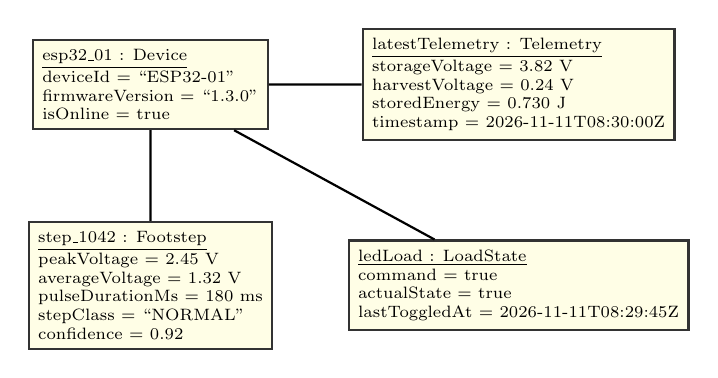
\begin{tikzpicture}[
    scale=0.85, every node/.style={scale=0.85},
    obj/.style={rectangle, draw=black!80, thick, fill=yellow!10, align=left, font=\scriptsize, inner sep=4pt}
]
    \node (dev1) [obj] at (0, 3) {
        \underline{esp32\_01 : Device}\\
        deviceId = ``ESP32-01''\\
        firmwareVersion = ``1.3.0''\\
        isOnline = true
    };

    \node (telem1) [obj] at (5.5, 3) {
        \underline{latestTelemetry : Telemetry}\\
        storageVoltage = 3.82 V\\
        harvestVoltage = 0.24 V\\
        storedEnergy = 0.730 J\\
        timestamp = 2026-11-11T08:30:00Z
    };

    \node (step1) [obj] at (0, 0) {
        \underline{step\_1042 : Footstep}\\
        peakVoltage = 2.45 V\\
        averageVoltage = 1.32 V\\
        pulseDurationMs = 180 ms\\
        stepClass = ``NORMAL''\\
        confidence = 0.92
    };

    \node (load1) [obj] at (5.5, 0) {
        \underline{ledLoad : LoadState}\\
        command = true\\
        actualState = true\\
        lastToggledAt = 2026-11-11T08:29:45Z
    };

    \draw [thick] (dev1) -- (telem1);
    \draw [thick] (dev1) -- (step1);
    \draw [thick] (dev1) -- (load1);

\end{tikzpicture}
\caption{Object Diagram capturing runtime instances during a footstep event.}
\label{fig:object_diagram}
\end{figure}
